\chapter{Statistics}
\label{stat}
For the next four question we use data from Tradeview taken from coinbase going back to 2016 to the present day. After cleaning the data the head is a follows
\begin{verbatim}
			time	open	high	low	close	Volume	range
date_time							
2016-05-23 10:00:00	1463961600	13.91	13.91	13.61	13.61	0.78673	0.30
2016-05-24 10:00:00	1464048000	13.68	13.74	12.00	12.77	2753.23998	1.74
2016-05-25 10:00:00	1464134400	13.00	13.18	11.93	12.61	9697.18313	1.25
2016-05-26 10:00:00	1464220800	12.61	12.95	12.15	12.47	2989.89229	0.80
2016-05-27 10:00:00	1464307200	12.47	12.47	10.25	10.98	19334.80484	2.22
\end{verbatim}

\section{ What is the average daily range.}
Summary statistics for range.

\begin{verbatim}
count    1565.000000
mean       21.331188
std        34.627367
min         0.100000
25%         4.440000
50%        11.080000
75%        24.380000
max       433.570000
\end{verbatim}
The average daily range is 21.331188. Figure \ref{fig:range} shows the range distribution.
\begin{figure}
\center
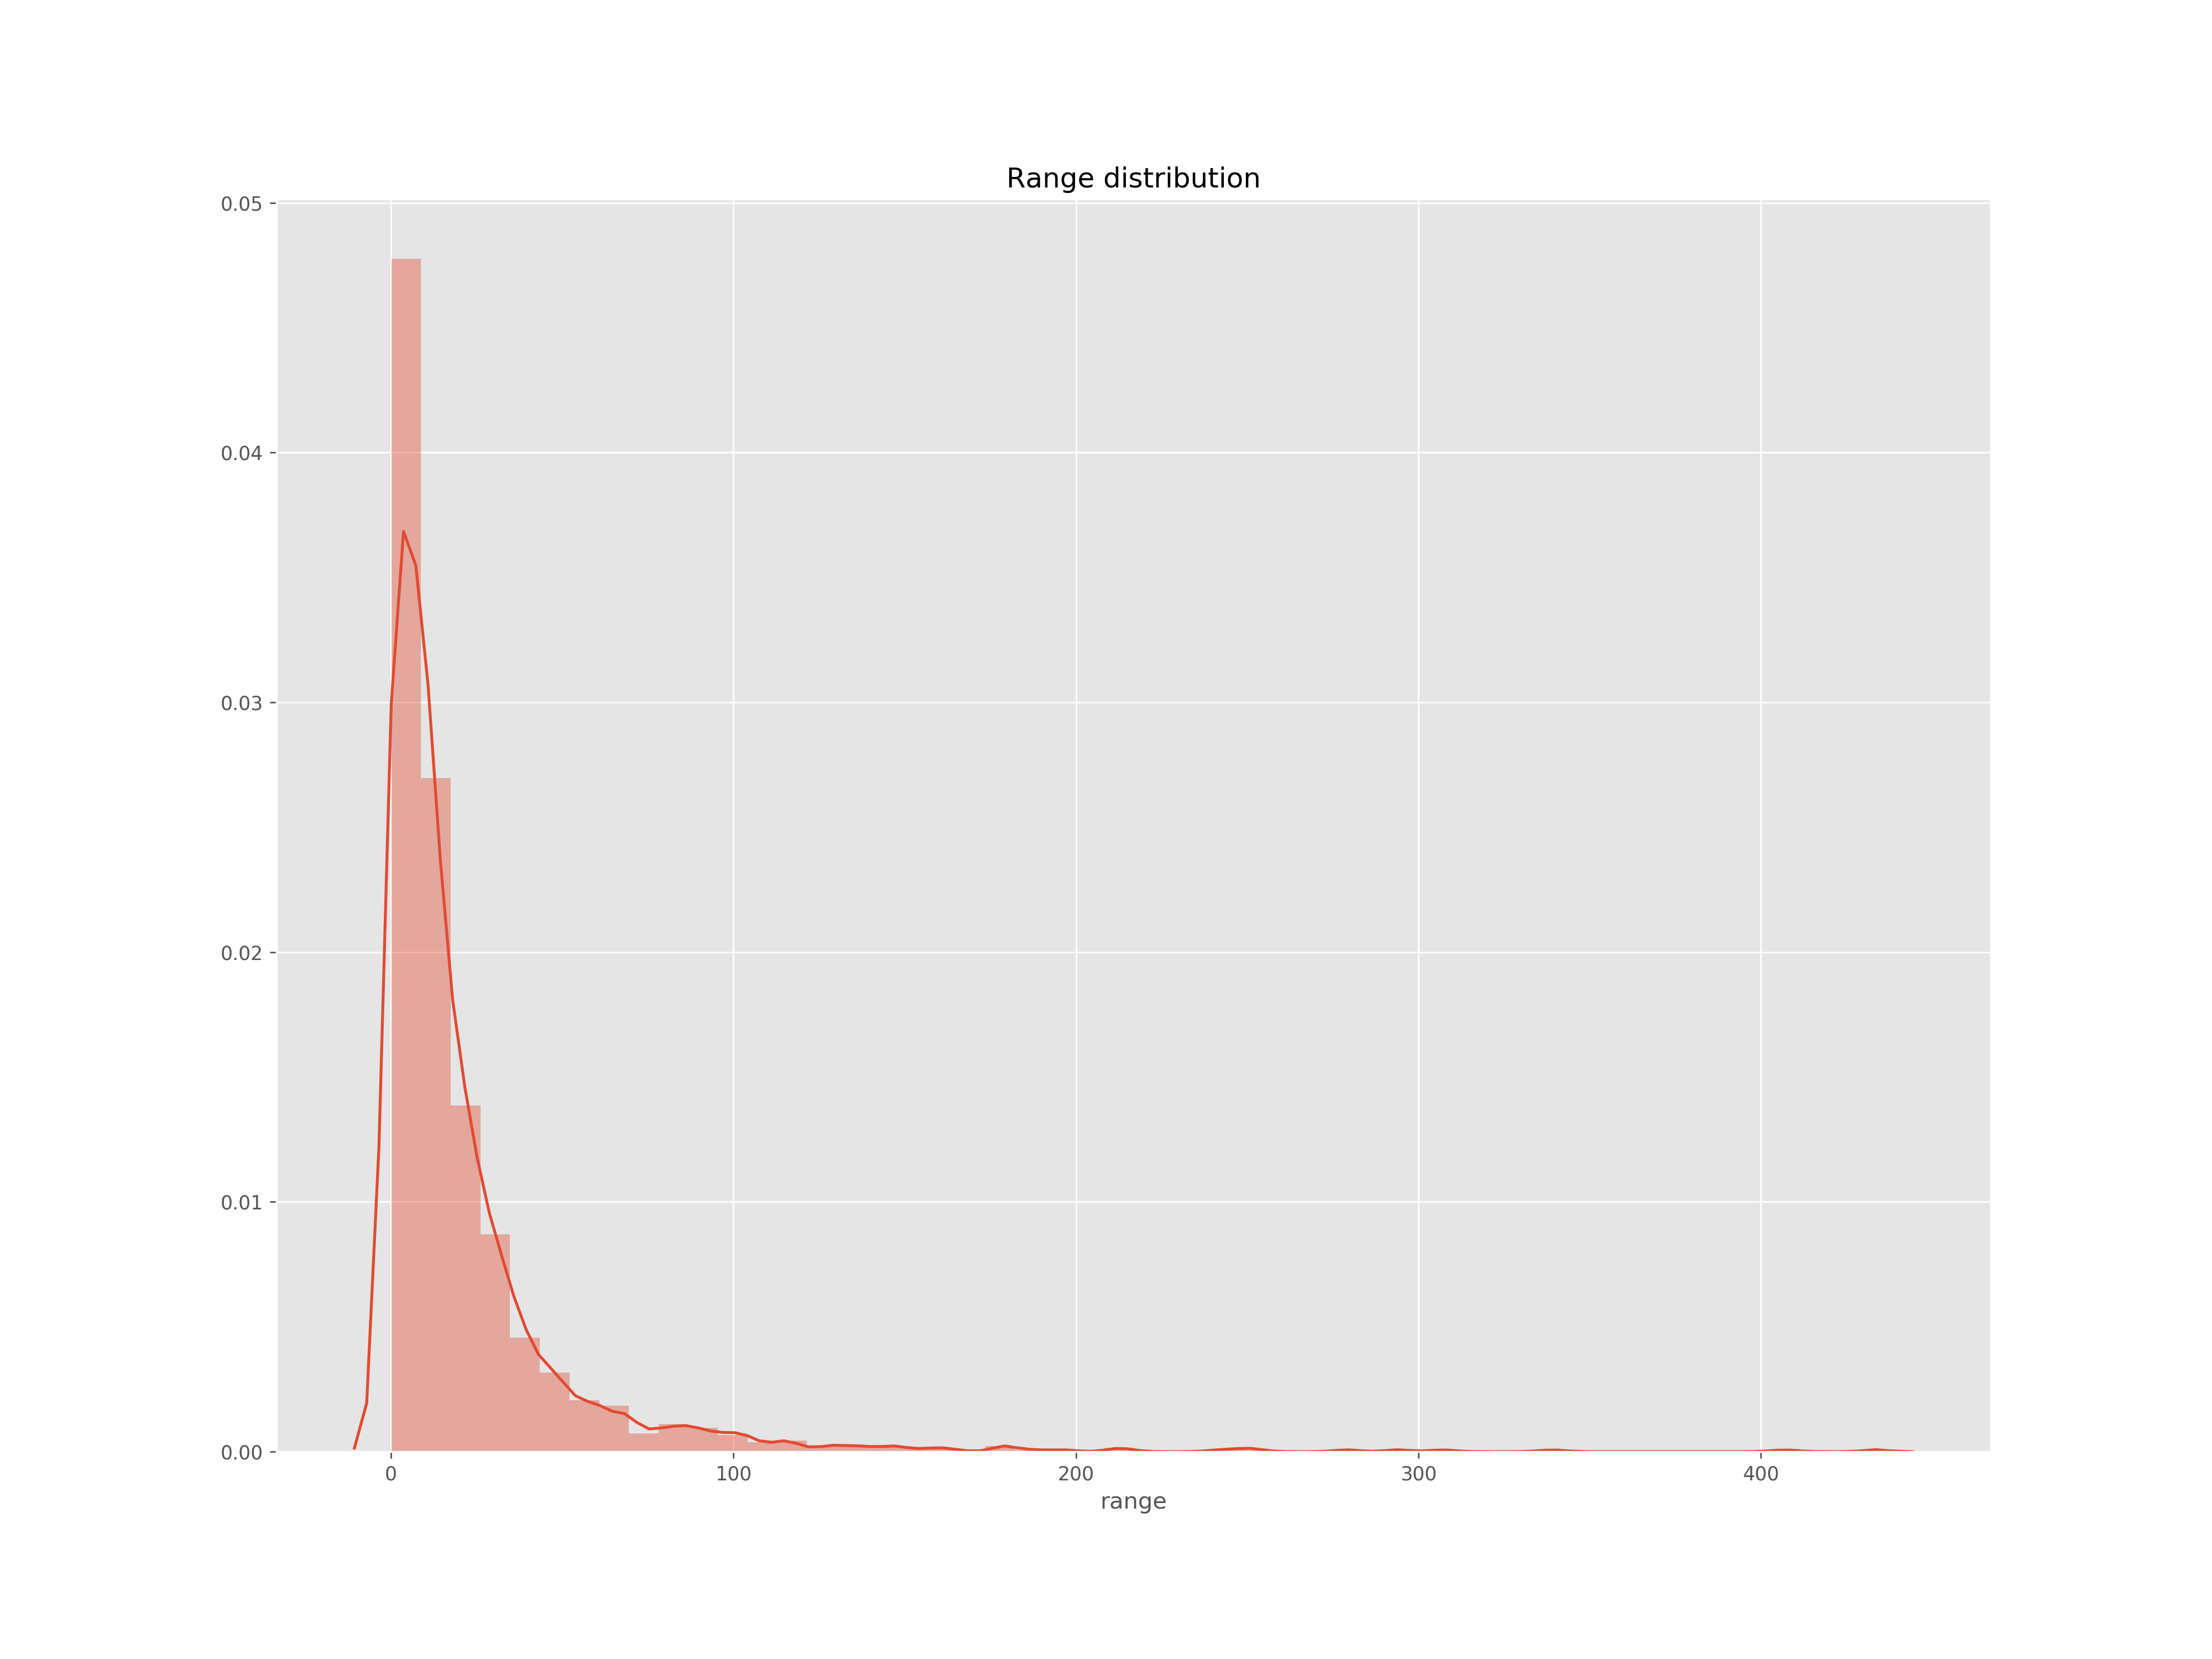
\includegraphics[width=0.9\textwidth]{fig/range.png}
\caption{Range distribution}
\label{fig:range}
\end{figure}

\section{ What is the average daily volume.}
Summary statistics for Volume.

\begin{verbatim}
count    1.565000e+03
mean     1.333461e+05
std      1.276997e+05
min      7.867300e-01
25%      5.343518e+04
50%      9.512464e+04
75%      1.669171e+05
max      1.322283e+06
\end{verbatim}
The average daily Volume is 1.333461e+05. Figure \ref{fig:vol_dist} shows the volume distribution.
\begin{figure}
\center
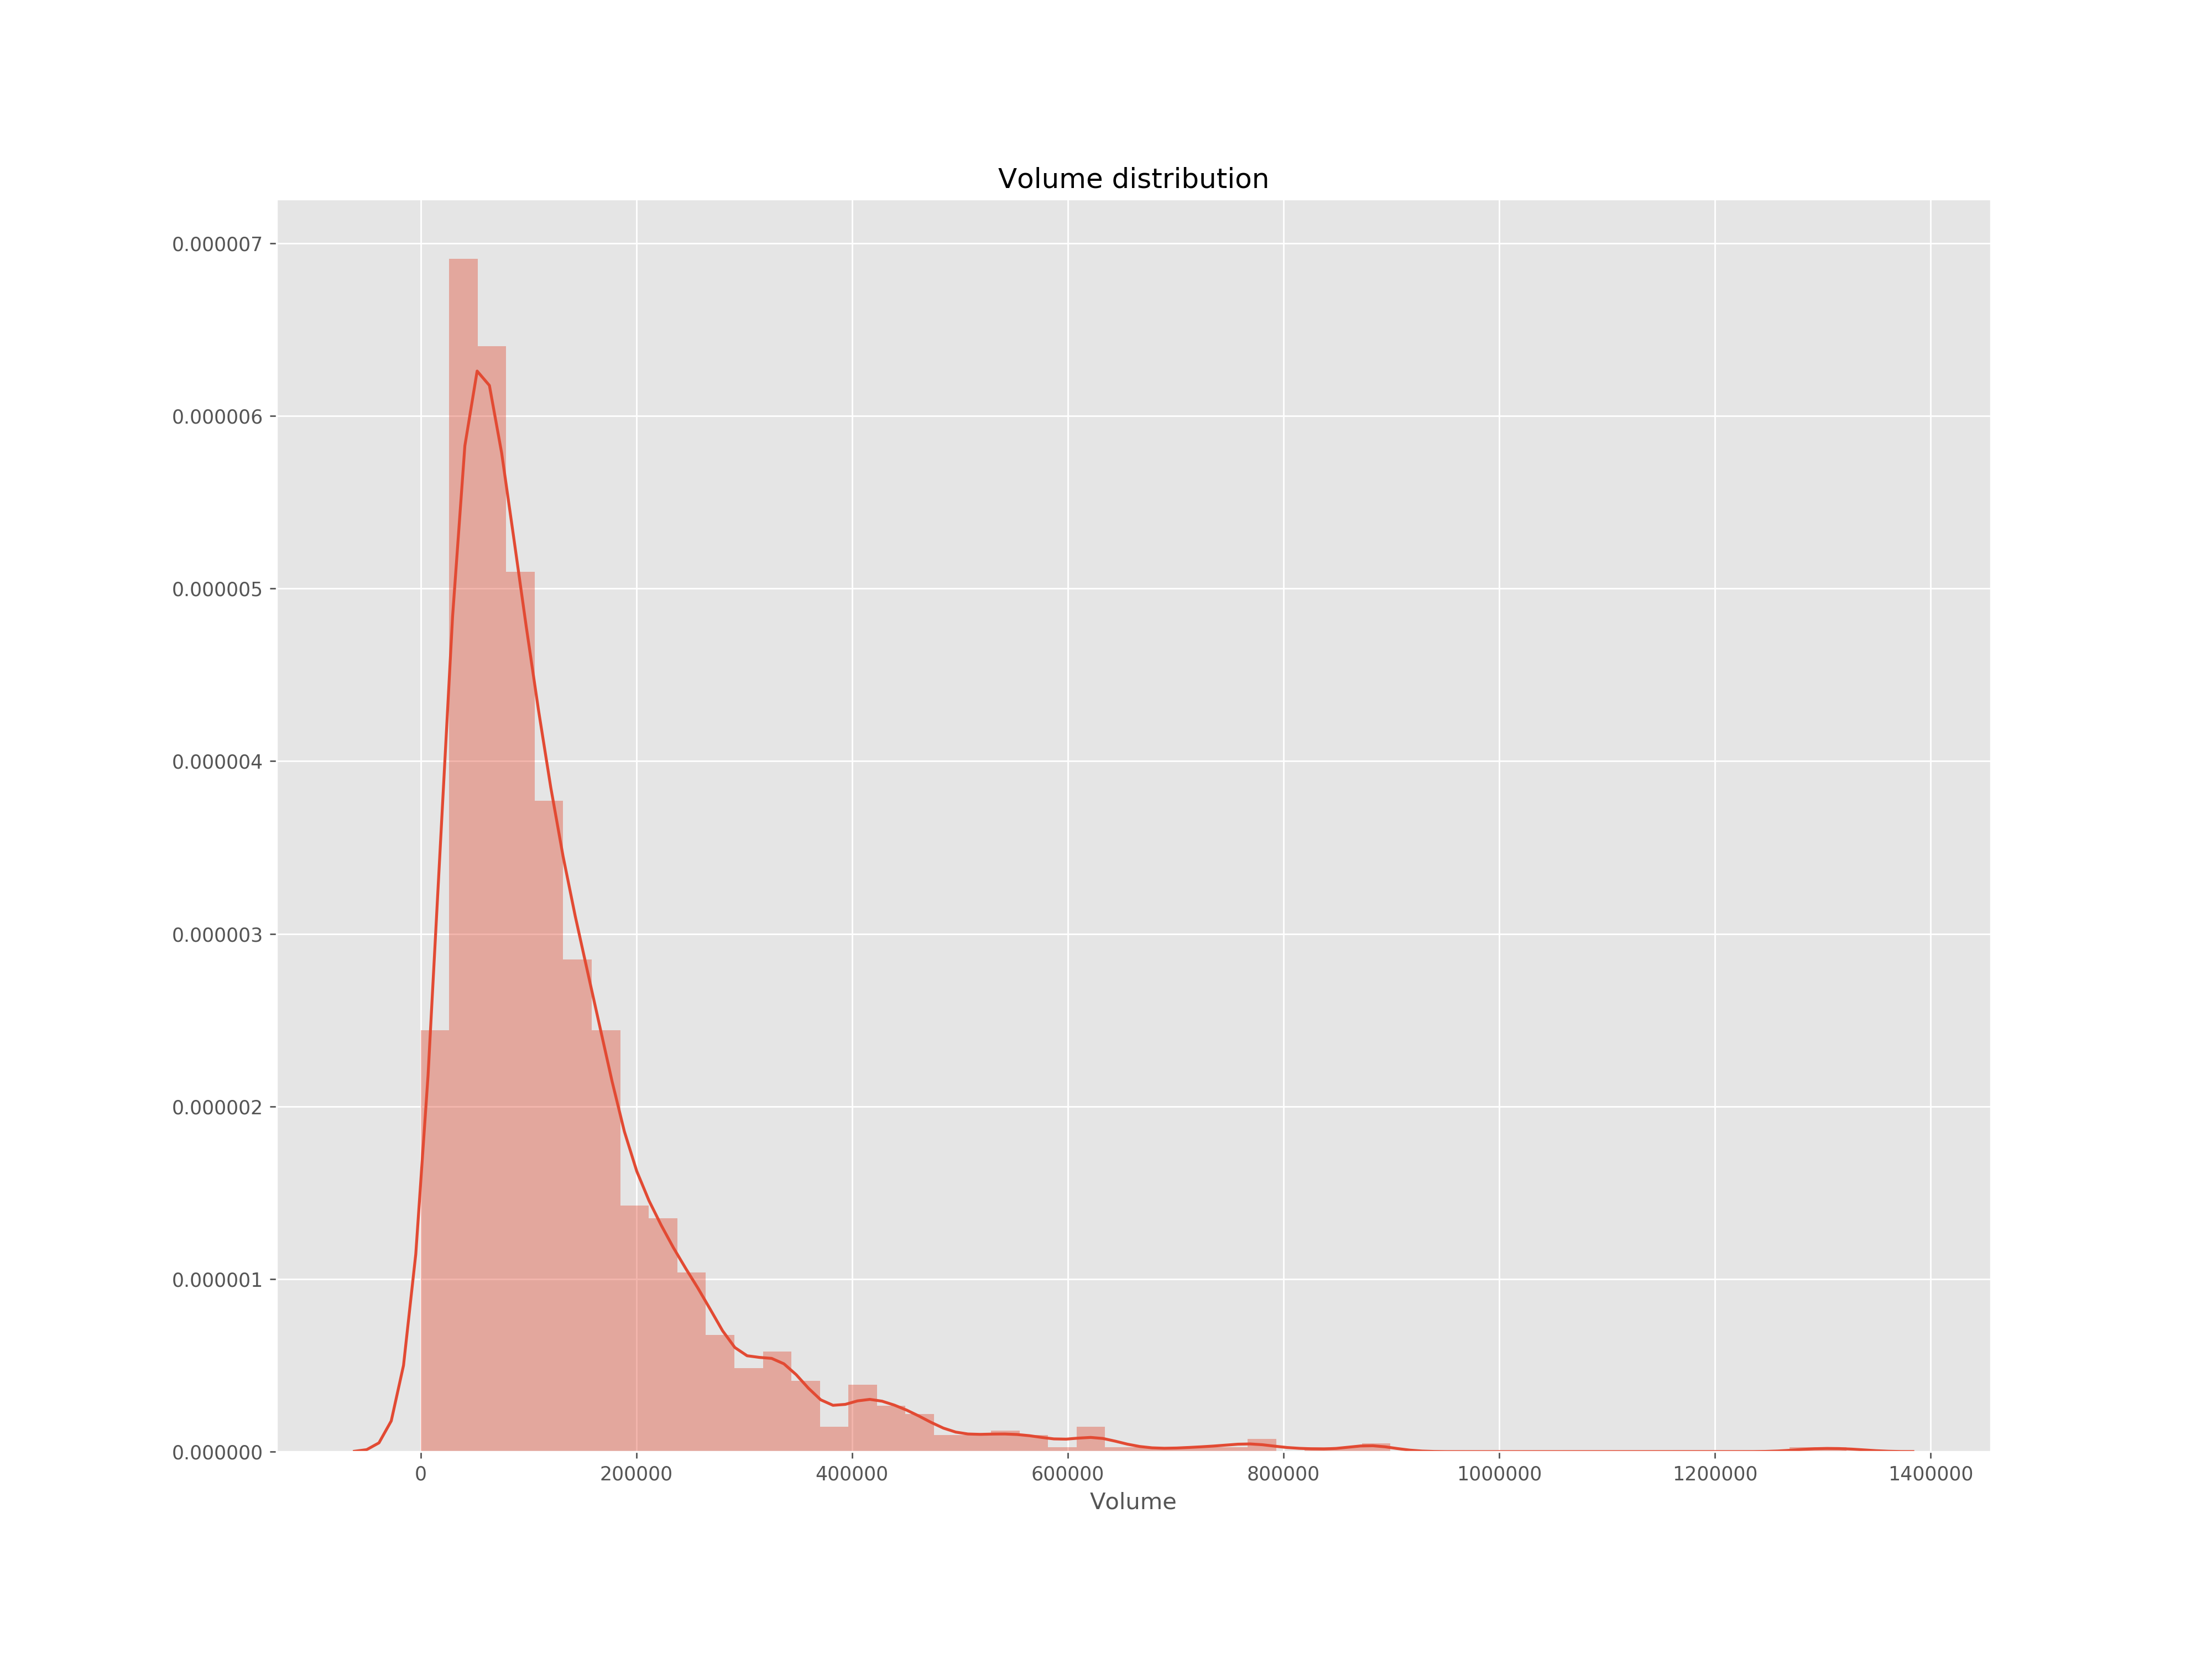
\includegraphics[width=0.9\textwidth]{fig/vol_dist.png}
\caption{Volume distribution}
\label{fig:vol_dist}
\end{figure}
\section{ What would you define as a low volume days?}
We will define volume below the 25th percentile to have low volume. Thus, a day with volume below 5.343518e+04 is low.
\section{ What is the average weekend range.}
The data is grouped by day of the week. 0 = Monday,..., 6= Sunday. 

The summary statstics for the groups are

\begin{tabular}{lrrrrrrr}
\toprule
{} &        time &        open &        high &         low &       close &         Volume &      range \\
day &             &             &             &             &             &                &            \\
\midrule
0   &  1531396800 &  244.666652 &  254.059286 &  233.163839 &  244.640179 &  139691.779979 &  20.895446 \\
1   &  1531483200 &  244.642768 &  254.736205 &  231.990179 &  245.165446 &  145372.288791 &  22.746027 \\
2   &  1531569600 &  245.172812 &  255.199821 &  230.065089 &  243.928795 &  150107.028572 &  25.134732 \\
3   &  1531656000 &  243.915134 &  253.779531 &  231.644643 &  242.454085 &  151790.895260 &  22.134888 \\
4   &  1531440000 &  241.549215 &  251.391749 &  229.833072 &  243.245695 &  141879.322847 &  21.558677 \\
5   &  1531526400 &  243.247578 &  253.825830 &  236.150538 &  246.119417 &  100524.152772 &  17.675291 \\
6   &  1531612800 &  246.120852 &  254.312287 &  235.164081 &  245.684126 &  103816.814631 &  19.148206 \\
\bottomrule
\end{tabular}

Thus the average weekend range

$$\frac{17.675291+ 19.148206}{2} = 18.4117485$$

In addition we plot the boxplots of ranges per day give by Figure \ref{fig:rday}. There is no evidence to suggest weekends range more. 
\begin{figure}
\center
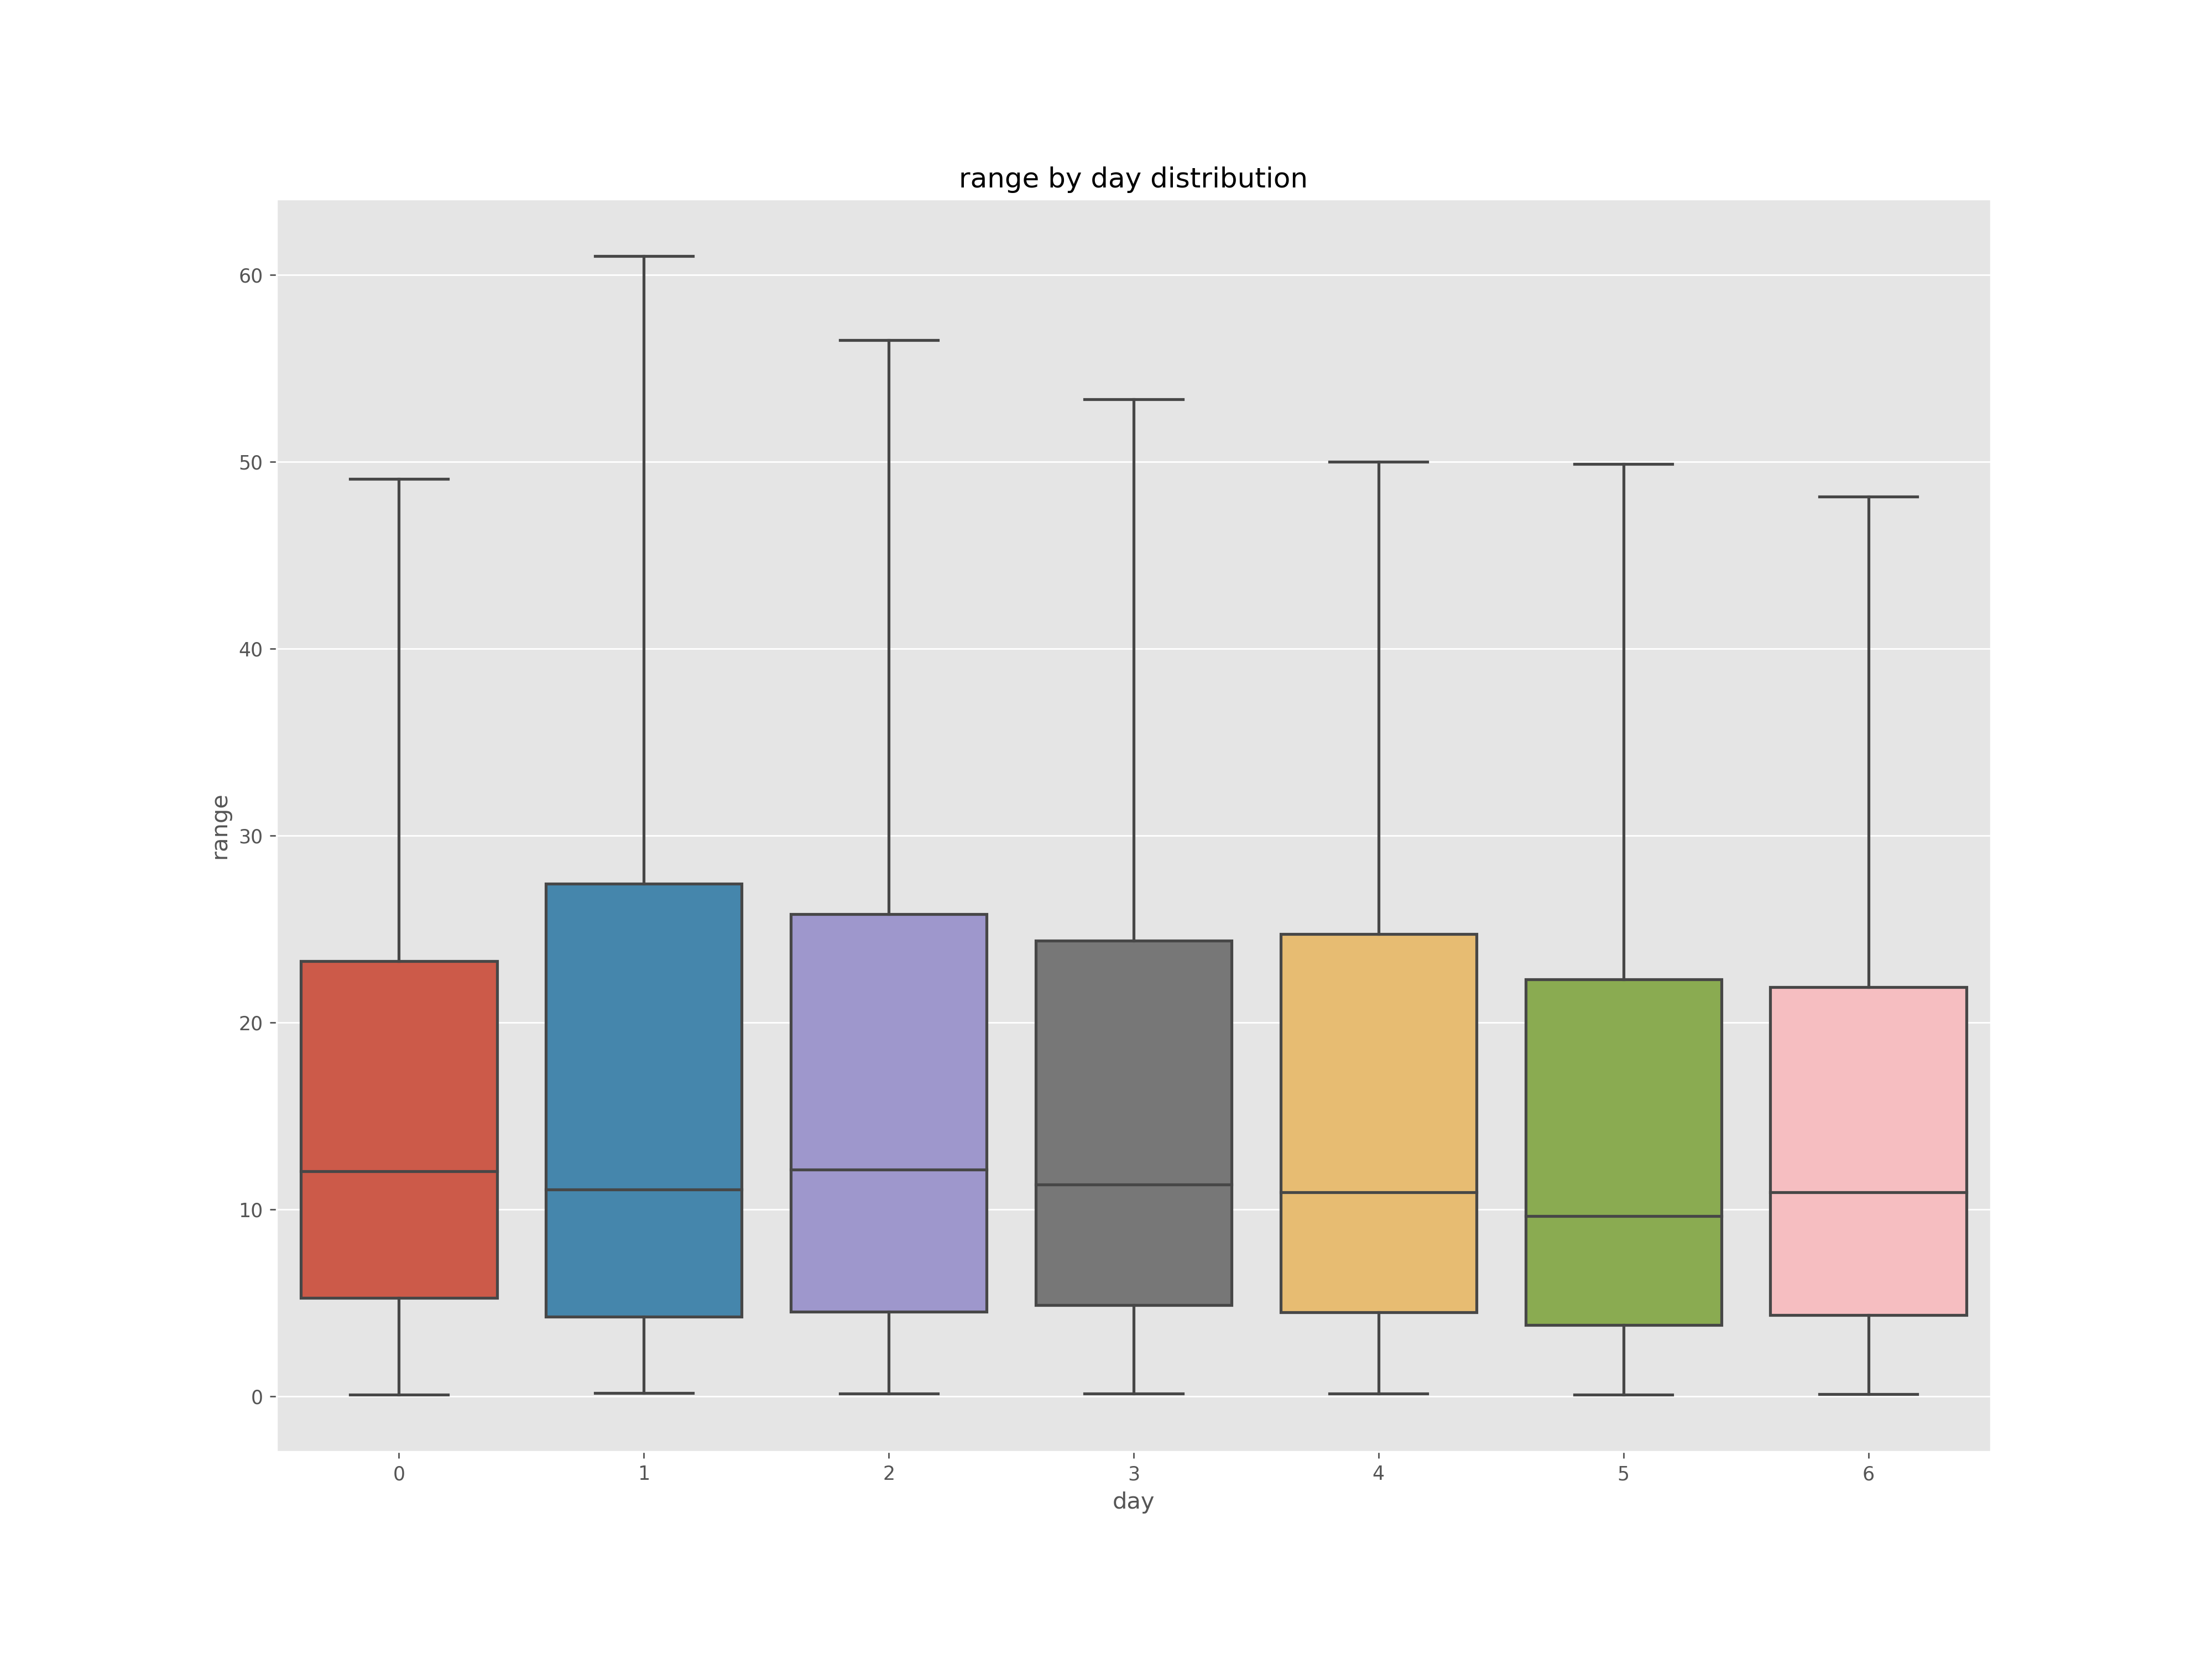
\includegraphics[width=0.9\textwidth]{fig/rday.png}
\caption{Range box plots by day}
\label{fig:rday}
\end{figure}
\section{ What affect does an increase in open interest have on price?}
cfgh
\section{ What affect does a decrease in open interest have on price?}
fgb
\section{ Does any relationship exist between open interest and price?}
fgnb



\section{ What is the average session range and volume - asia euro usa.}


We define the asia, usa, euro session in UTC time.

\begin{verbatim}
exchange_times = {
    'asia': [time(),time(hour = 6)],
    'usa': [time(hour=13,minute=30),time(hour = 20)],
    'euro': [time(hour=8),time(hour=16,minute=30)],   
}
\end{verbatim}
The \texttt{time()} is the amount of time past $00:00$ UTC. For example \texttt{time(hour=13,minute=30)} is $13:30$ UTC.

We perform the following on a data set for the past 3 years from coinbase with an hourly resolution. Note that there were rate limits on the api so 88 separate http requests had to sent.

\begin{itemize}
\item data was categorised into asia, usa, euro sessions
\item For session it was resampled to daily data
\end{itemize}

This yielded the following statistics  for volume and range

\begin{verbatim}
For the asia session
             range        volume
count  1100.000000   1100.000000
mean      5.053318   7559.744723
std       7.499806   7136.945473
min       0.292857    798.873352
25%       1.608571   3196.329492
50%       2.829286   5258.516808
75%       5.315714   9015.883759
max      84.672857  55962.362899
----------------------------------------------------
For the usa session
             range        volume
count  1100.000000   1100.000000
mean      4.340860   4472.978179
std       6.641011   4877.610076
min       0.190000    407.690536
25%       1.266786   1813.502618
50%       2.240000   3046.332611
75%       4.462143   5280.163938
max      75.645714  62737.359162
----------------------------------------------------
For the euro session
             range         volume
count  1101.000000    1101.000000
mean      4.691296    6347.743122
std       7.187887    6717.636049
min       0.212222     692.604705
25%       1.443333    2548.551281
50%       2.537778    4424.716103
75%       4.984444    7611.190454
max     106.830000  102992.740244
\end{verbatim}

\section{ Work out the ATR of Eth in excel and read the ATR pdf.}
Here is the python code that computes the 14 period ATR. 
\begin{verbatim}
x = 14
df_ATR[f"atr_period_{x}"] = df_ATR["range"]
for i in range(1,x):
    df_ATR[f"atr_period_{x}"] = df_ATR[f"atr_period_{x}"] +  df_ATR[f"atr_period_{x}"].shift(i)
df_ATR[f"atr_period_{x}"]  = df_ATR[f"atr_period_{x}"]/df_ATR["open"].shift(x-1)

df_ATR.plot(figsize=(12,8))

plt.title("14 period ATR distribution")
plt.savefig("../../../report/fig/atr.png",dpi=250)
plt.show()
\end{verbatim}



\begin{figure}
\center
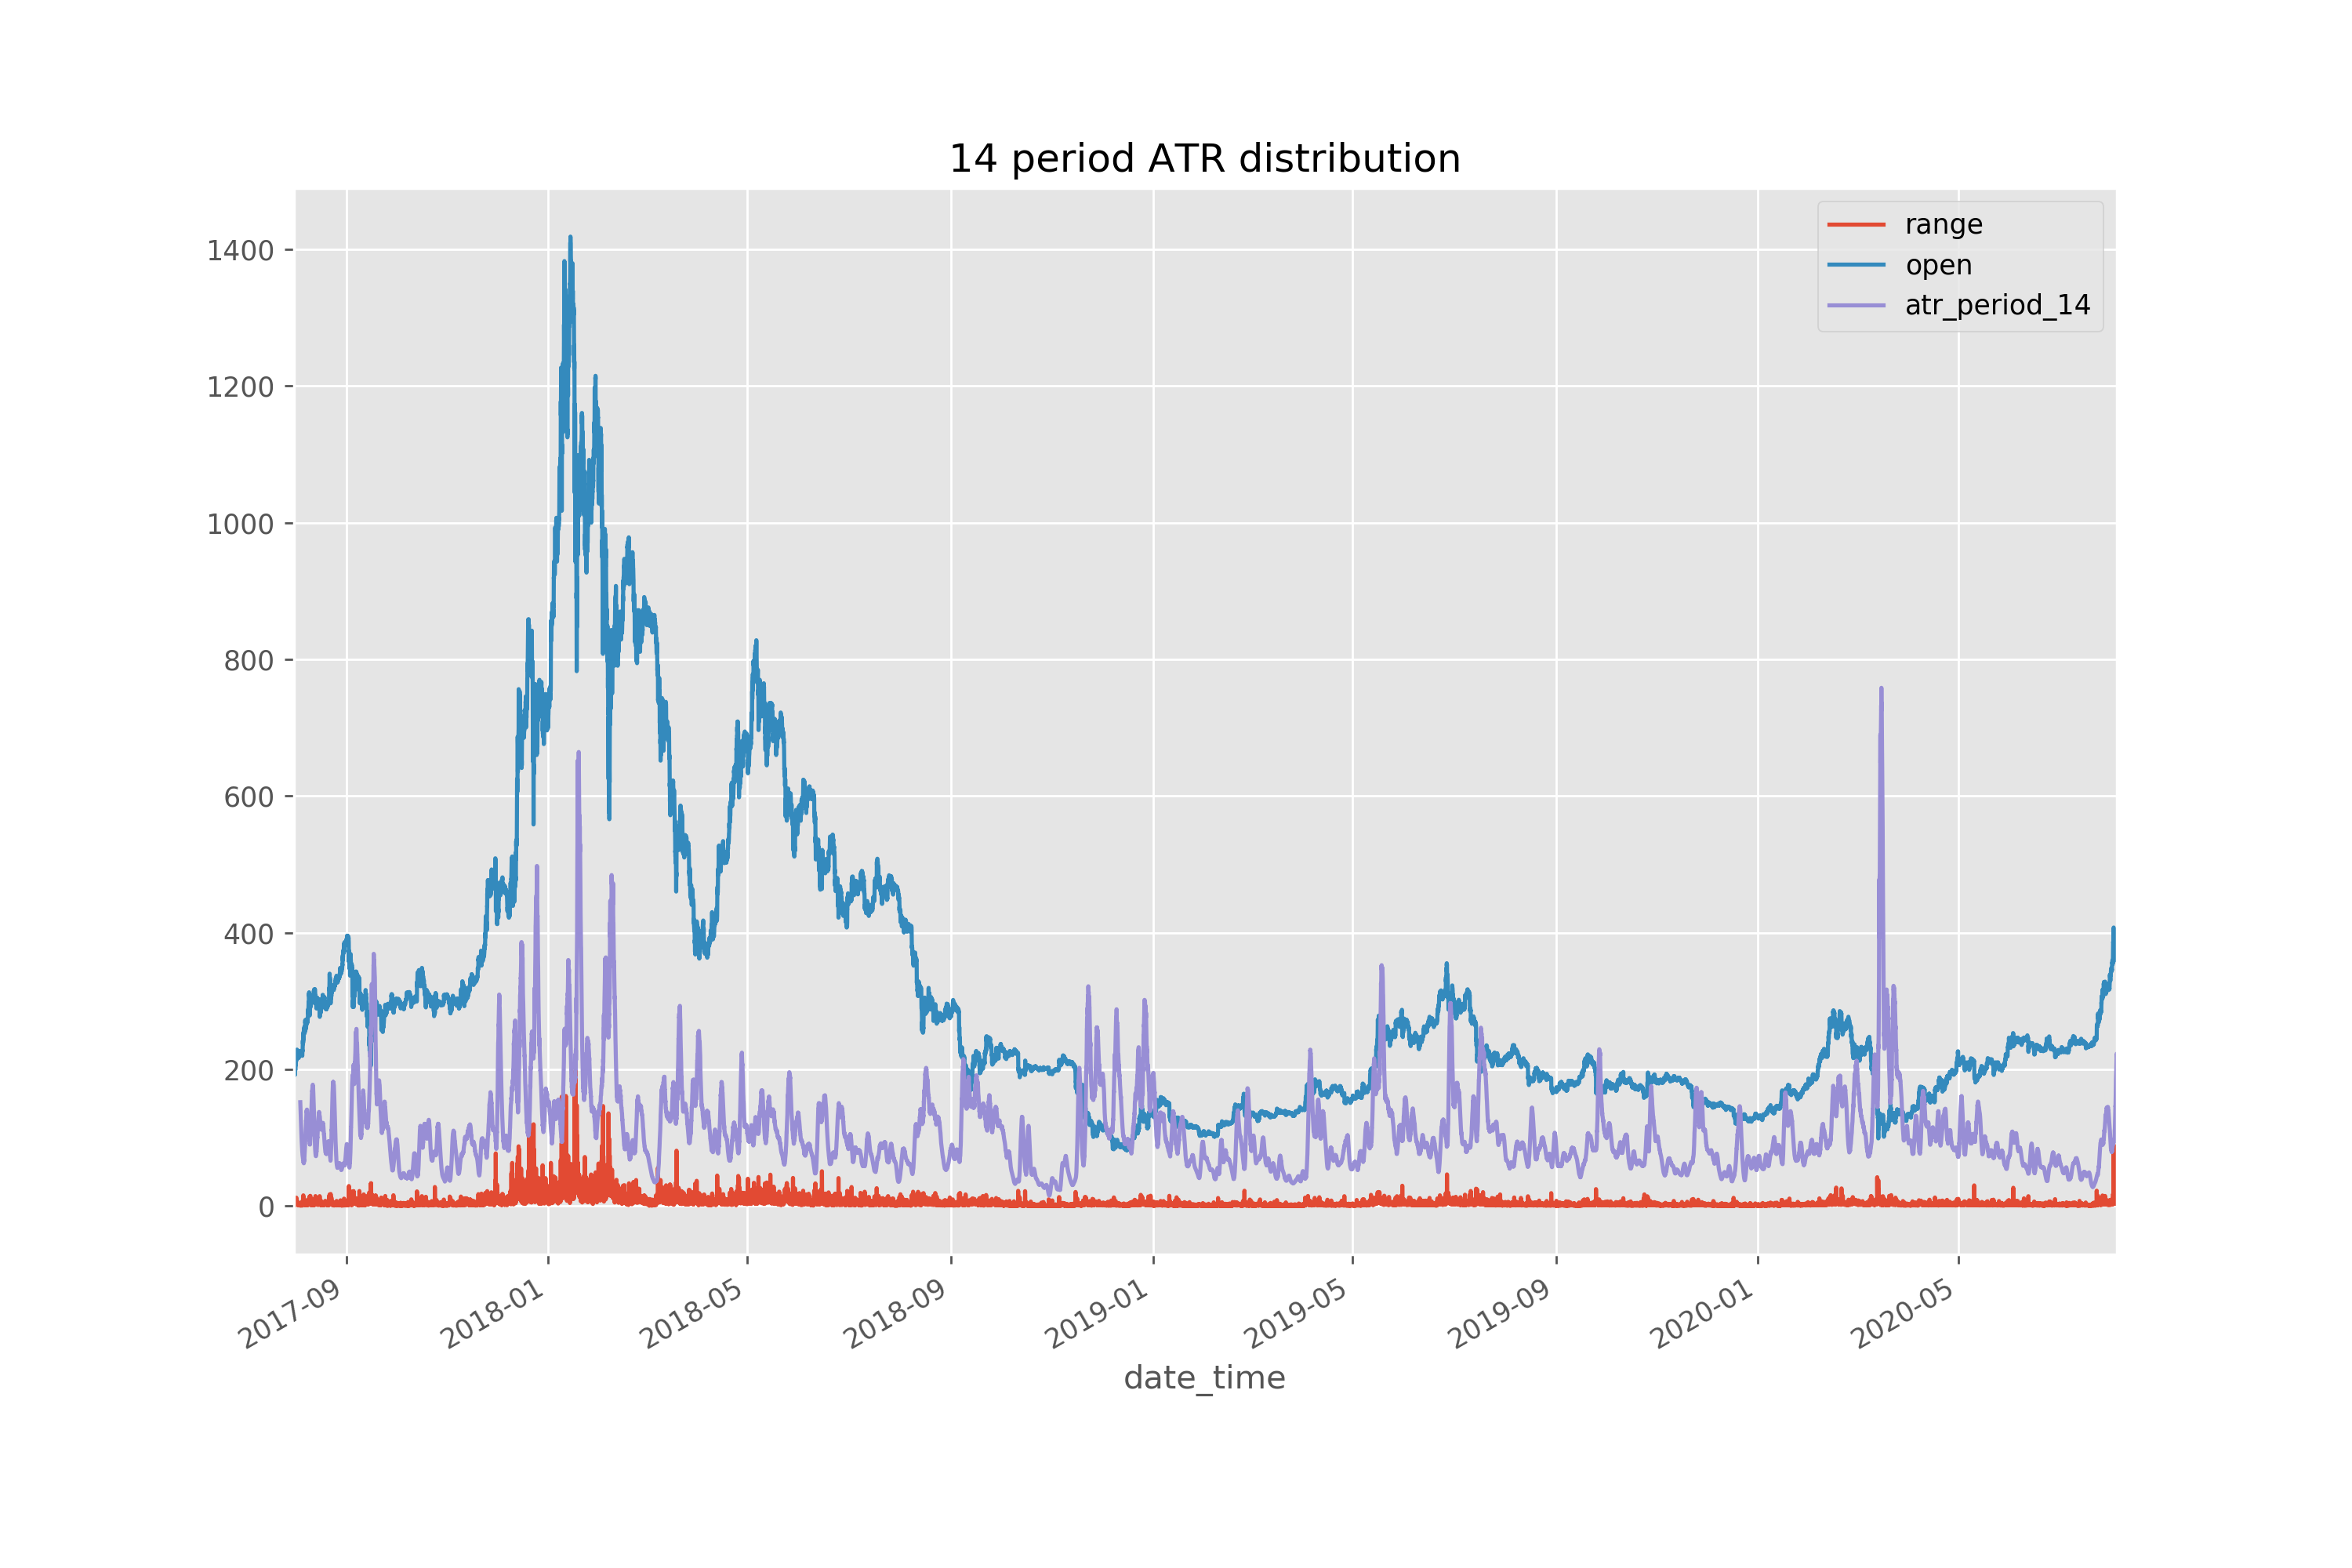
\includegraphics[width=0.9\textwidth]{fig/atr.png}
\caption{14 period ATR for 3 years of hourly data on ETHUSD}
\label{fig:atr}
\end{figure}
Figure \ref{fig:atr} plots the ATR along with the range and open.


\section{ Work out the distribution of returns and read the pdf.}
The summary statistic for the returns distribution
\begin{verbatim}
count    26387.000000
mean         0.000090
std          0.011256
min         -0.196000
25%         -0.003853
50%          0.000060
75%          0.004015
max          0.183455
\end{verbatim}

\begin{figure}
\center
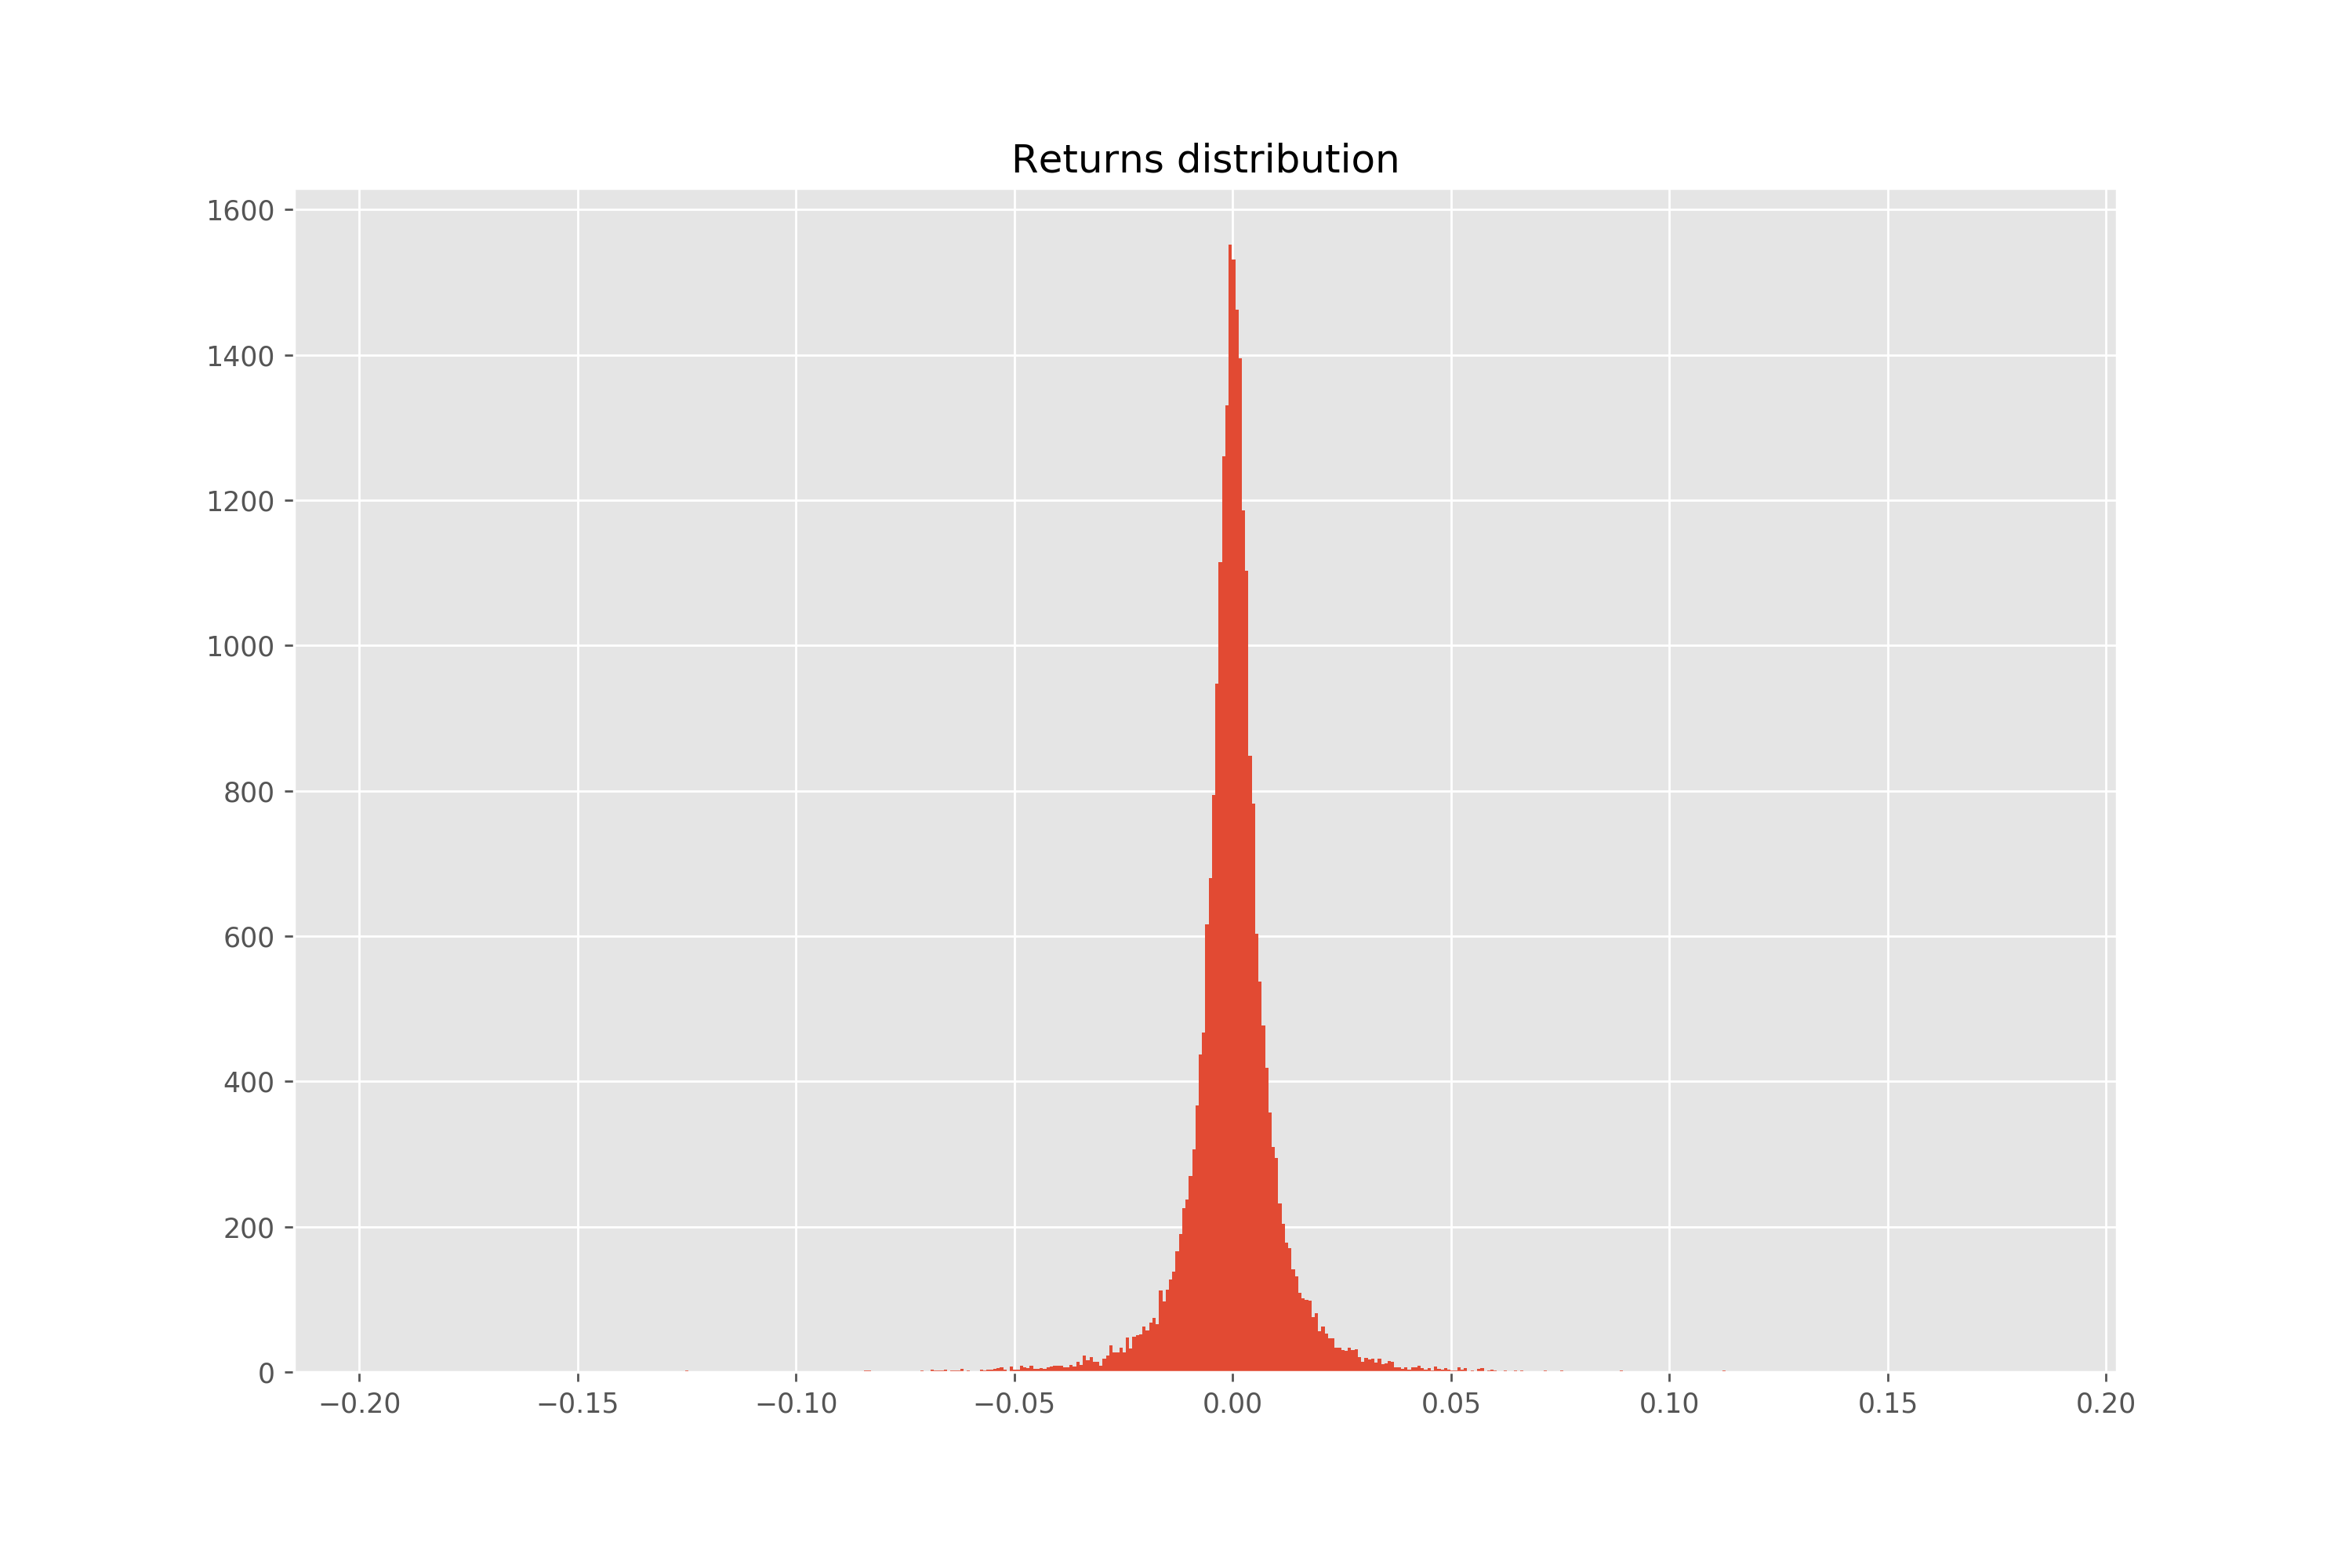
\includegraphics[width=0.9\textwidth]{fig/ret.png}
\caption{Returns for 3 years of hourly data on ETHUSD}
\label{fig:ret}
\end{figure}


\section{ What is the most common time of day for price movements.}

Figure \ref{fig:pm} shows price movements by time of day. A higher variance means a higher price move. Thus, price moves the most at 2:00 UTC.
\begin{figure}
\center
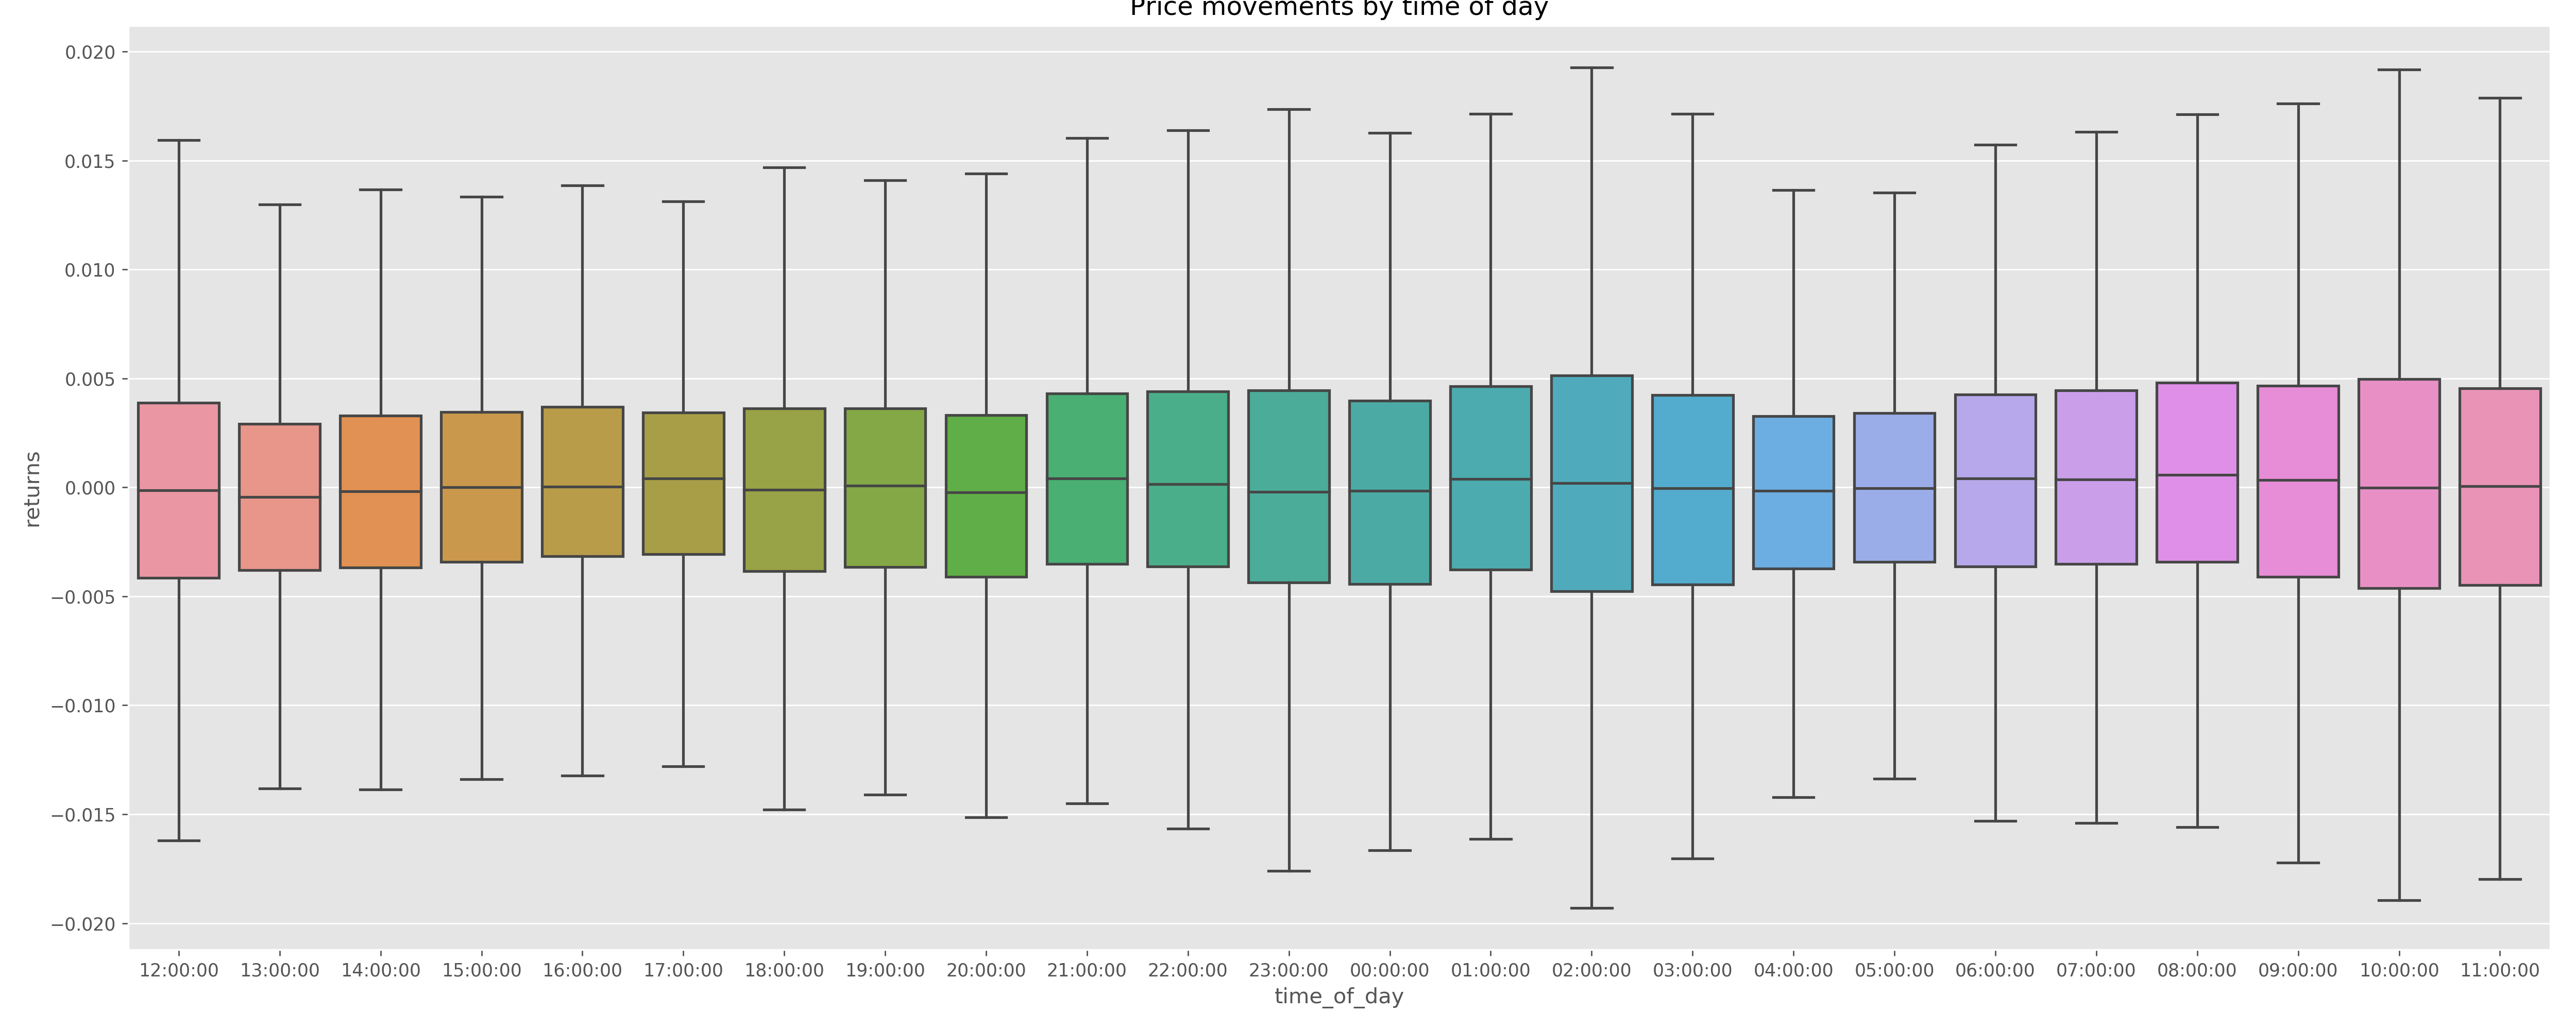
\includegraphics[width=0.9\textwidth]{fig/pm.png}
\caption{Price movements by time of day for 3 years of hourly data on ETHUSD}
\label{fig:pm}
\end{figure}
 
\section{ What are the most common times with the most volume.}
Figure \ref{fig:vol_times} shows volume by time of day. Thus, most volume is at 2:00 and 3:00 UTC.
\begin{figure}
\center
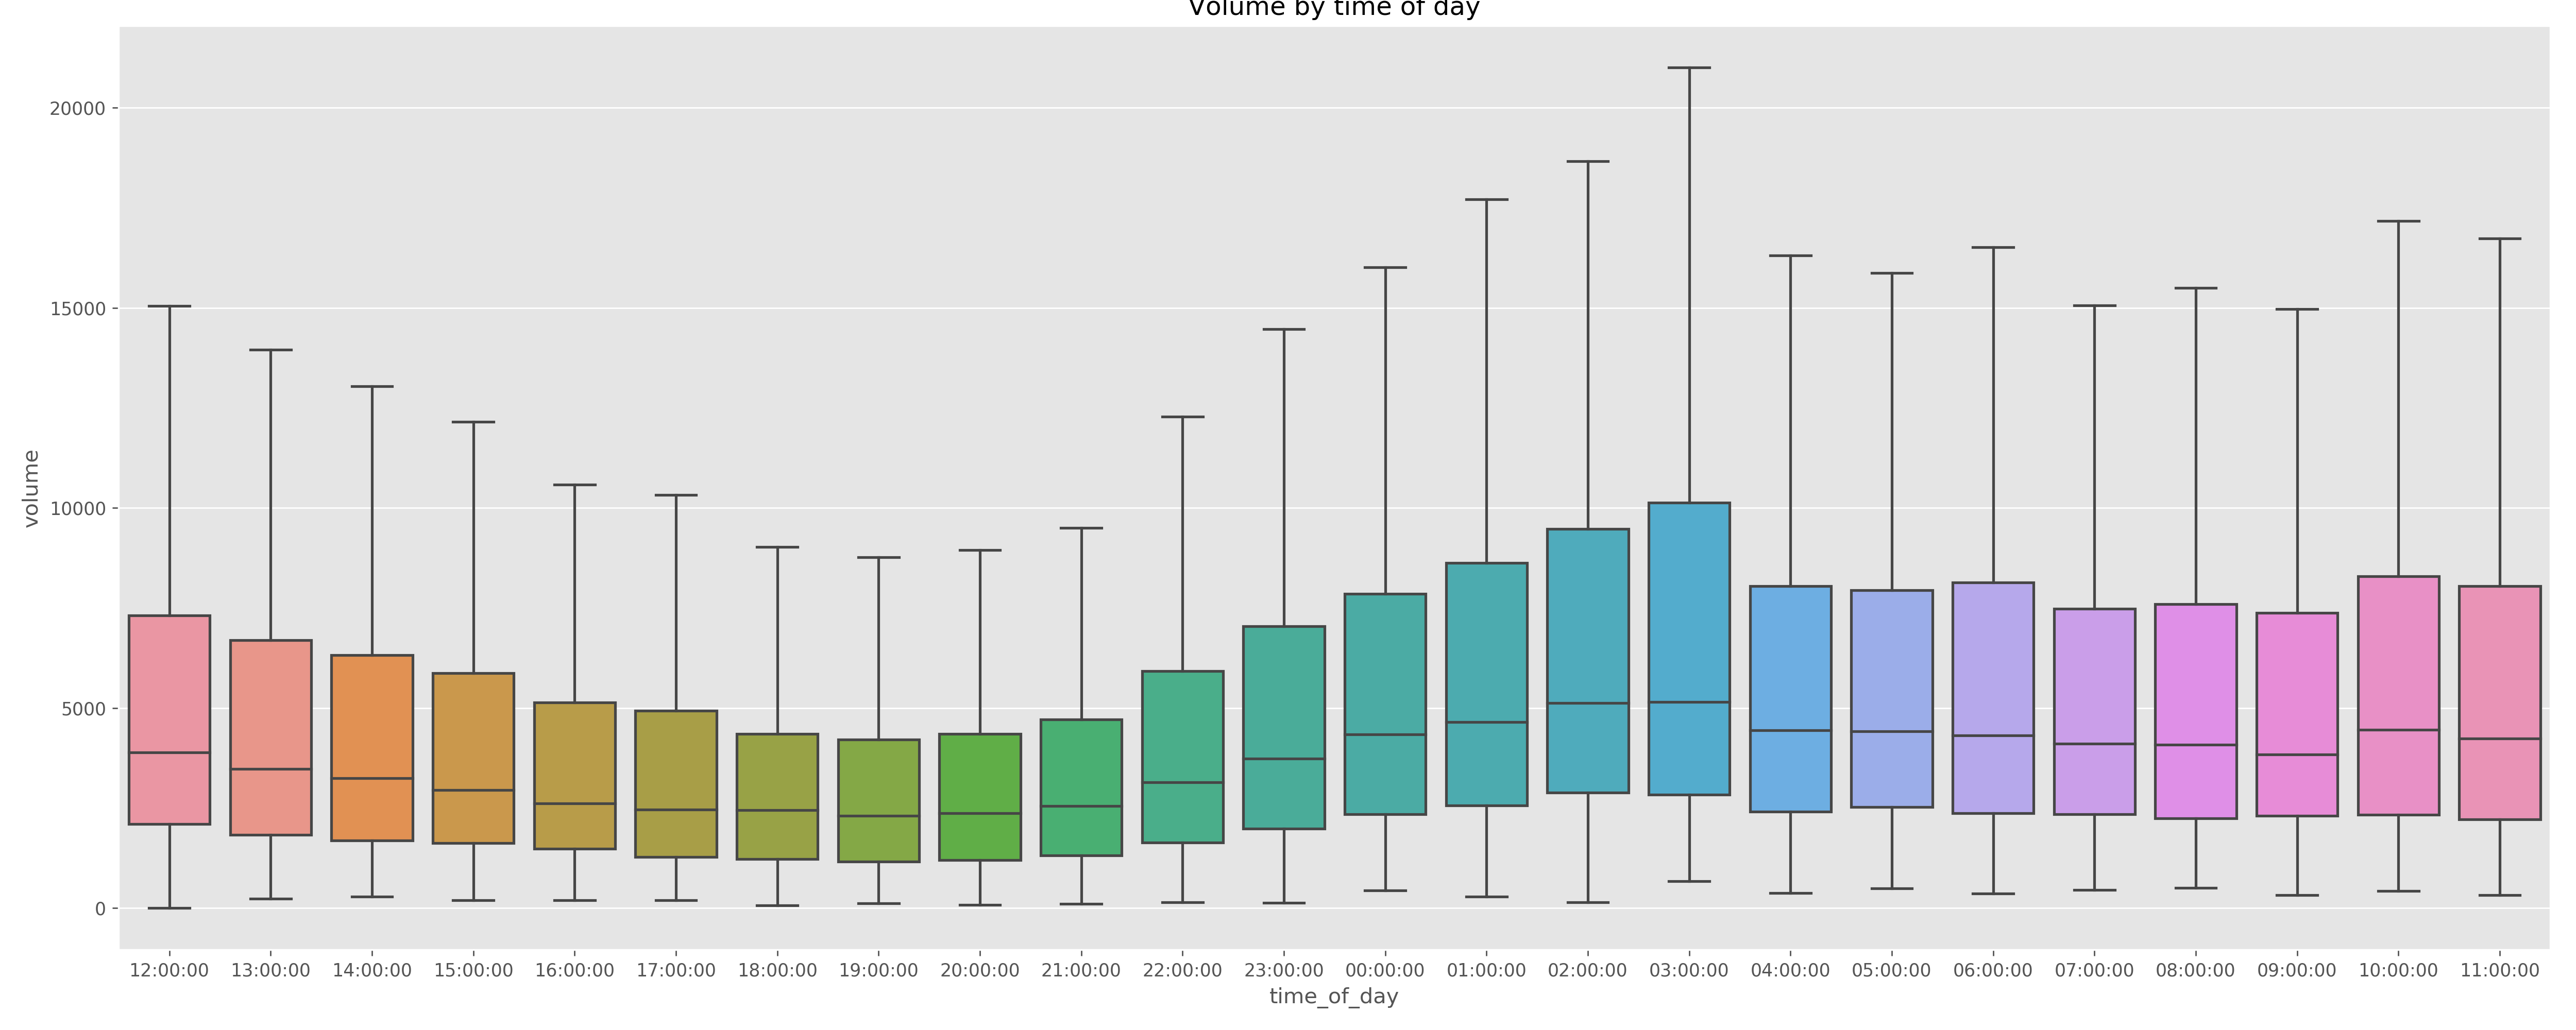
\includegraphics[width=0.9\textwidth]{fig/vol_times.png}
\caption{Volume by time of day for 3 years of hourly data on ETHUSD}
\label{fig:vol_times}
\end{figure}

\section{ Is beginning of the month typically quieter then end of month?}
Figure \ref{fig:qt} shows volume by day of the month. Thus, most volume is in the middle of the month. The start and the end of the month have roughly the same volume.
\begin{figure}
\center
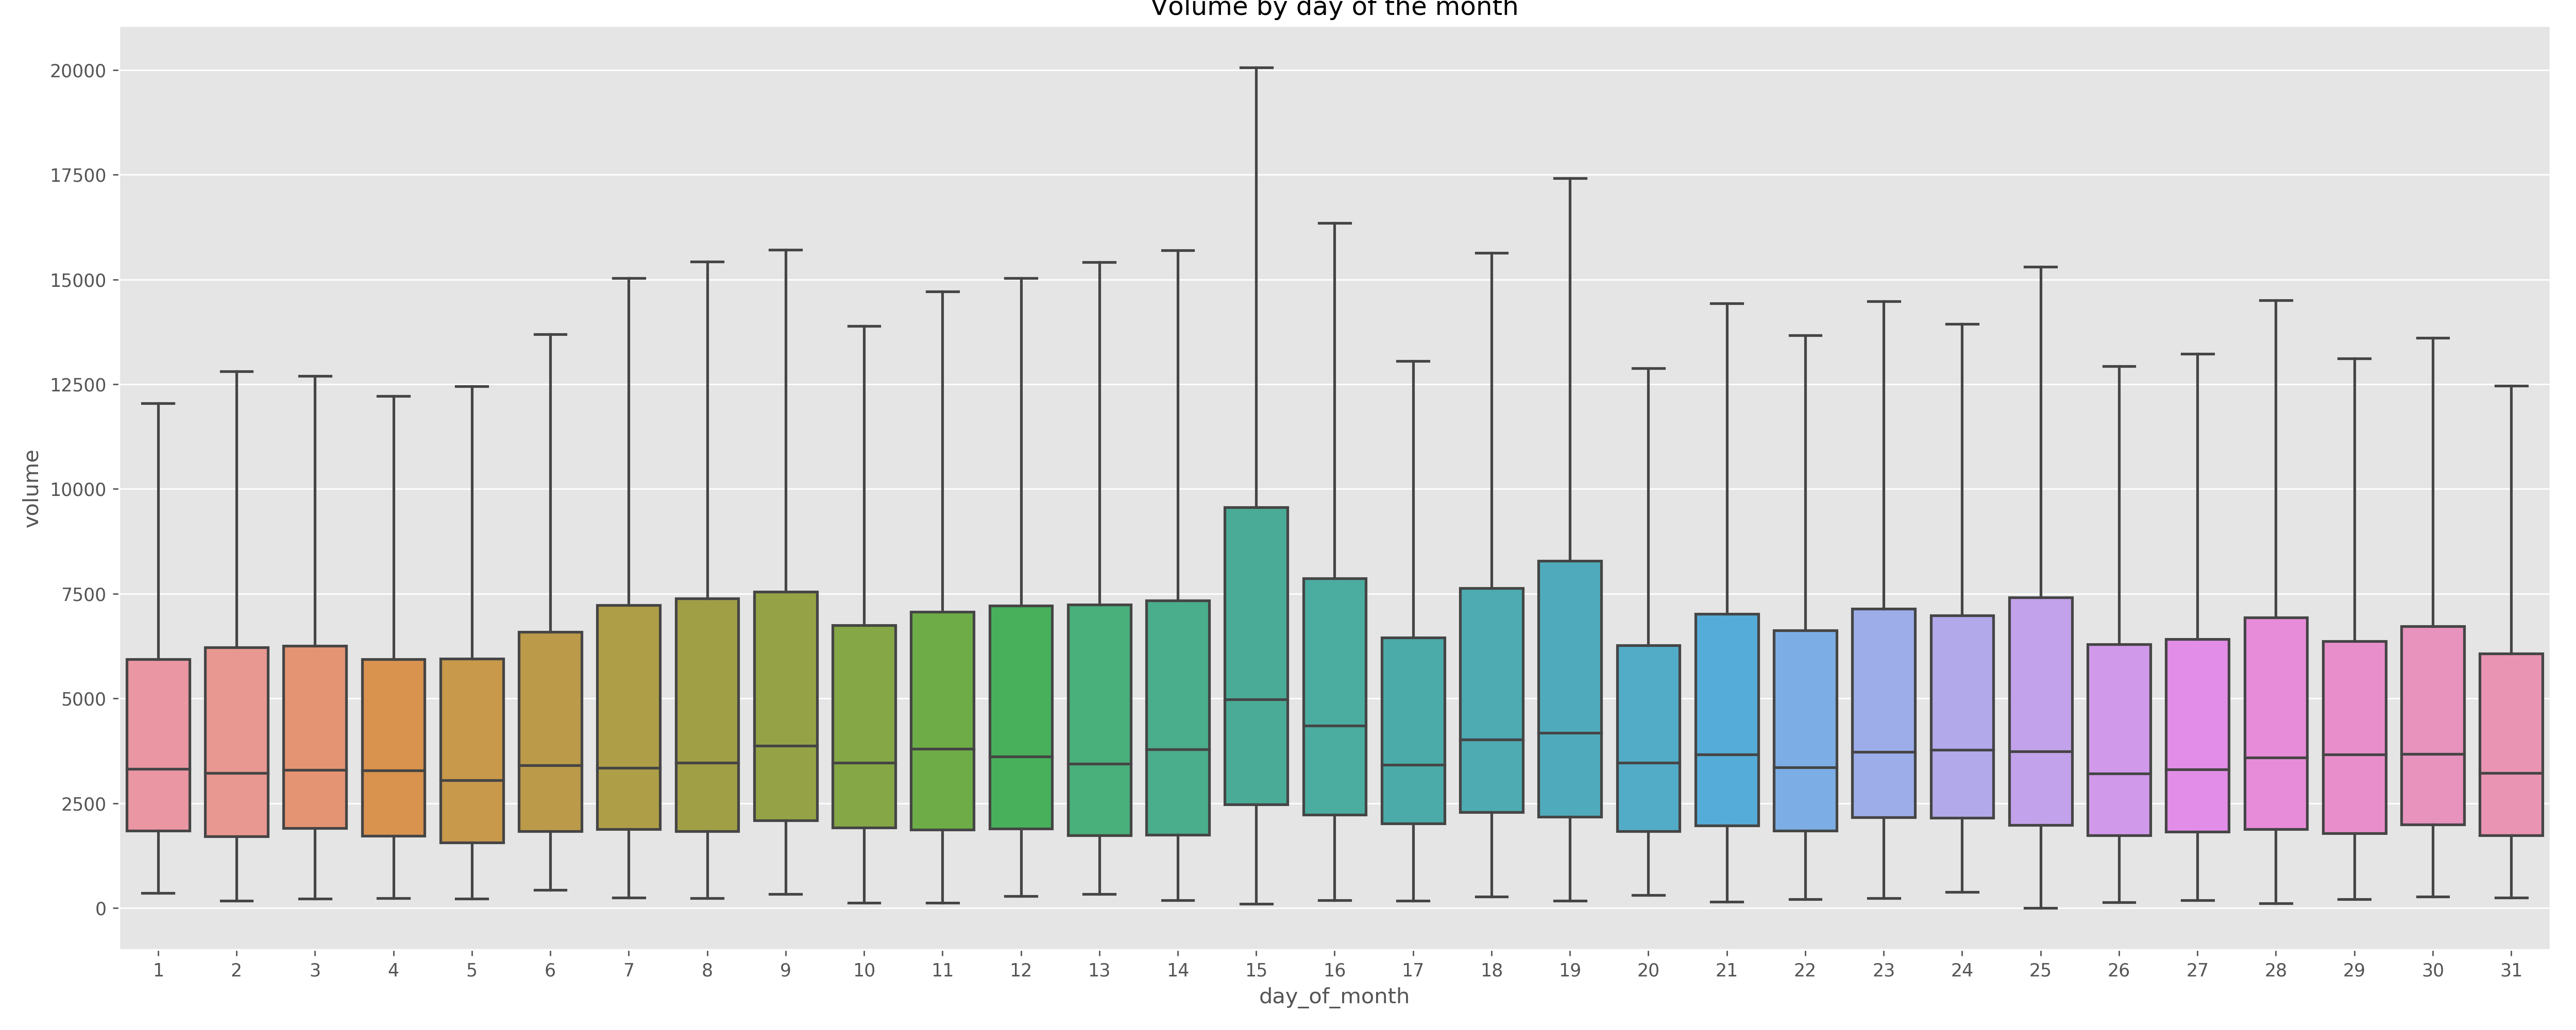
\includegraphics[width=0.9\textwidth]{fig/qt.png}
\caption{Volume by time of day for 3 years of hourly data on ETHUSD}
\label{fig:qt}
\end{figure}

\section{ List of days where it trades greater then its Standard deviation, check (1SD, 2SD, 3SD)}
Using z scores of the resampled daily return we have

\begin{verbatim}
For days between 1 and 2 SD
[Timestamp('2017-08-01 00:00:00'),
 Timestamp('2017-08-02 00:00:00'),
 Timestamp('2017-08-07 00:00:00'),
 Timestamp('2017-08-17 00:00:00'),
 Timestamp('2017-08-21 00:00:00'),
 Timestamp('2017-08-30 00:00:00'),
 Timestamp('2017-09-03 00:00:00'),
 Timestamp('2017-09-06 00:00:00'),
 Timestamp('2017-09-09 00:00:00'),
 Timestamp('2017-09-13 00:00:00'),
 Timestamp('2017-09-14 00:00:00'),
 Timestamp('2017-09-17 00:00:00'),
 Timestamp('2017-09-19 00:00:00'),
 Timestamp('2017-09-22 00:00:00'),
 Timestamp('2017-09-24 00:00:00'),
 Timestamp('2017-09-28 00:00:00'),
 Timestamp('2017-10-18 00:00:00'),
 Timestamp('2017-11-09 00:00:00'),
 Timestamp('2017-11-11 00:00:00'),
 Timestamp('2017-12-01 00:00:00'),
 Timestamp('2017-12-02 00:00:00'),
 Timestamp('2017-12-07 00:00:00'),
 Timestamp('2017-12-15 00:00:00'),
 Timestamp('2017-12-23 00:00:00'),
 Timestamp('2017-12-24 00:00:00'),
 Timestamp('2017-12-26 00:00:00'),
 Timestamp('2017-12-28 00:00:00'),
 Timestamp('2018-01-02 00:00:00'),
 Timestamp('2018-01-03 00:00:00'),
 Timestamp('2018-01-04 00:00:00'),
 Timestamp('2018-01-05 00:00:00'),
 Timestamp('2018-01-07 00:00:00'),
 Timestamp('2018-01-12 00:00:00'),
 Timestamp('2018-01-13 00:00:00'),
 Timestamp('2018-01-14 00:00:00'),
 Timestamp('2018-01-16 00:00:00'),
 Timestamp('2018-01-18 00:00:00'),
 Timestamp('2018-01-19 00:00:00'),
 Timestamp('2018-01-21 00:00:00'),
 Timestamp('2018-01-22 00:00:00'),
 Timestamp('2018-01-23 00:00:00'),
 Timestamp('2018-01-25 00:00:00'),
 Timestamp('2018-01-28 00:00:00'),
 Timestamp('2018-01-29 00:00:00'),
 Timestamp('2018-01-31 00:00:00'),
 Timestamp('2018-02-03 00:00:00'),
 Timestamp('2018-02-08 00:00:00'),
 Timestamp('2018-02-10 00:00:00'),
 Timestamp('2018-02-11 00:00:00'),
 Timestamp('2018-02-15 00:00:00'),
 Timestamp('2018-02-21 00:00:00'),
 Timestamp('2018-02-22 00:00:00'),
 Timestamp('2018-03-07 00:00:00'),
 Timestamp('2018-03-08 00:00:00'),
 Timestamp('2018-03-09 00:00:00'),
 Timestamp('2018-03-23 00:00:00'),
 Timestamp('2018-03-29 00:00:00'),
 Timestamp('2018-04-05 00:00:00'),
 Timestamp('2018-04-20 00:00:00'),
 Timestamp('2018-04-21 00:00:00'),
 Timestamp('2018-04-26 00:00:00'),
 Timestamp('2018-04-27 00:00:00'),
 Timestamp('2018-05-03 00:00:00'),
 Timestamp('2018-05-07 00:00:00'),
 Timestamp('2018-05-11 00:00:00'),
 Timestamp('2018-05-12 00:00:00'),
 Timestamp('2018-05-14 00:00:00'),
 Timestamp('2018-05-23 00:00:00'),
 Timestamp('2018-05-28 00:00:00'),
 Timestamp('2018-05-29 00:00:00'),
 Timestamp('2018-05-30 00:00:00'),
 Timestamp('2018-06-11 00:00:00'),
 Timestamp('2018-06-13 00:00:00'),
 Timestamp('2018-06-15 00:00:00'),
 Timestamp('2018-06-22 00:00:00'),
 Timestamp('2018-06-23 00:00:00'),
 Timestamp('2018-06-27 00:00:00'),
 Timestamp('2018-07-03 00:00:00'),
 Timestamp('2018-07-10 00:00:00'),
 Timestamp('2018-07-11 00:00:00'),
 Timestamp('2018-07-18 00:00:00'),
 Timestamp('2018-08-01 00:00:00'),
 Timestamp('2018-08-08 00:00:00'),
 Timestamp('2018-08-09 00:00:00'),
 Timestamp('2018-08-16 00:00:00'),
 Timestamp('2018-08-18 00:00:00'),
 Timestamp('2018-08-19 00:00:00'),
 Timestamp('2018-08-21 00:00:00'),
 Timestamp('2018-09-12 00:00:00'),
 Timestamp('2018-09-19 00:00:00'),
 Timestamp('2018-09-21 00:00:00'),
 Timestamp('2018-09-25 00:00:00'),
 Timestamp('2018-09-26 00:00:00'),
 Timestamp('2018-10-11 00:00:00'),
 Timestamp('2018-10-12 00:00:00'),
 Timestamp('2018-11-21 00:00:00'),
 Timestamp('2018-11-23 00:00:00'),
 Timestamp('2018-11-25 00:00:00'),
 Timestamp('2018-11-27 00:00:00'),
 Timestamp('2018-11-29 00:00:00'),
 Timestamp('2018-12-04 00:00:00'),
 Timestamp('2018-12-06 00:00:00'),
 Timestamp('2018-12-19 00:00:00'),
 Timestamp('2018-12-26 00:00:00'),
 Timestamp('2018-12-28 00:00:00'),
 Timestamp('2019-01-02 00:00:00'),
 Timestamp('2019-01-03 00:00:00'),
 Timestamp('2019-01-14 00:00:00'),
 Timestamp('2019-01-15 00:00:00'),
 Timestamp('2019-01-21 00:00:00'),
 Timestamp('2019-01-28 00:00:00'),
 Timestamp('2019-01-29 00:00:00'),
 Timestamp('2019-02-18 00:00:00'),
 Timestamp('2019-02-24 00:00:00'),
 Timestamp('2019-03-06 00:00:00'),
 Timestamp('2019-03-16 00:00:00'),
 Timestamp('2019-04-08 00:00:00'),
 Timestamp('2019-04-12 00:00:00'),
 Timestamp('2019-04-26 00:00:00'),
 Timestamp('2019-05-07 00:00:00'),
 Timestamp('2019-05-14 00:00:00'),
 Timestamp('2019-05-15 00:00:00'),
 Timestamp('2019-05-18 00:00:00'),
 Timestamp('2019-05-23 00:00:00'),
 Timestamp('2019-05-27 00:00:00'),
 Timestamp('2019-05-31 00:00:00'),
 Timestamp('2019-06-04 00:00:00'),
 Timestamp('2019-06-13 00:00:00'),
 Timestamp('2019-06-22 00:00:00'),
 Timestamp('2019-07-01 00:00:00'),
 Timestamp('2019-07-02 00:00:00'),
 Timestamp('2019-07-08 00:00:00'),
 Timestamp('2019-07-18 00:00:00'),
 Timestamp('2019-07-28 00:00:00'),
 Timestamp('2019-08-19 00:00:00'),
 Timestamp('2019-08-29 00:00:00'),
 Timestamp('2019-09-08 00:00:00'),
 Timestamp('2019-09-18 00:00:00'),
 Timestamp('2019-09-28 00:00:00'),
 Timestamp('2019-10-01 00:00:00'),
 Timestamp('2019-10-08 00:00:00'),
 Timestamp('2019-10-10 00:00:00'),
 Timestamp('2019-10-24 00:00:00'),
 Timestamp('2019-11-23 00:00:00'),
 Timestamp('2019-11-25 00:00:00'),
 Timestamp('2019-12-17 00:00:00'),
 Timestamp('2019-12-18 00:00:00'),
 Timestamp('2020-01-20 00:00:00'),
 Timestamp('2020-02-06 00:00:00'),
 Timestamp('2020-02-07 00:00:00'),
 Timestamp('2020-02-15 00:00:00'),
 Timestamp('2020-02-17 00:00:00'),
 Timestamp('2020-02-19 00:00:00'),
 Timestamp('2020-02-20 00:00:00'),
 Timestamp('2020-02-26 00:00:00'),
 Timestamp('2020-02-27 00:00:00'),
 Timestamp('2020-03-03 00:00:00'),
 Timestamp('2020-03-15 00:00:00'),
 Timestamp('2020-03-16 00:00:00'),
 Timestamp('2020-03-23 00:00:00'),
 Timestamp('2020-03-24 00:00:00'),
 Timestamp('2020-04-03 00:00:00'),
 Timestamp('2020-04-17 00:00:00'),
 Timestamp('2020-04-19 00:00:00'),
 Timestamp('2020-04-21 00:00:00'),
 Timestamp('2020-04-23 00:00:00'),
 Timestamp('2020-04-30 00:00:00'),
 Timestamp('2020-05-04 00:00:00'),
 Timestamp('2020-05-10 00:00:00'),
 Timestamp('2020-05-11 00:00:00'),
 Timestamp('2020-05-18 00:00:00'),
 Timestamp('2020-05-22 00:00:00'),
 Timestamp('2020-05-29 00:00:00'),
 Timestamp('2020-05-31 00:00:00'),
 Timestamp('2020-06-12 00:00:00'),
 Timestamp('2020-07-23 00:00:00'),
 Timestamp('2020-07-24 00:00:00'),
 Timestamp('2020-07-26 00:00:00'),
 Timestamp('2020-07-27 00:00:00'),
 Timestamp('2020-08-01 00:00:00'),
 Timestamp('2020-08-02 00:00:00')]
------------------------------------------------------------------------
For days between 2 and 3 SD
[Timestamp('2017-08-06 00:00:00'),
 Timestamp('2017-08-09 00:00:00'),
 Timestamp('2017-09-05 00:00:00'),
 Timestamp('2017-09-18 00:00:00'),
 Timestamp('2017-10-14 00:00:00'),
 Timestamp('2017-11-24 00:00:00'),
 Timestamp('2017-11-25 00:00:00'),
 Timestamp('2017-12-09 00:00:00'),
 Timestamp('2017-12-12 00:00:00'),
 Timestamp('2017-12-14 00:00:00'),
 Timestamp('2017-12-19 00:00:00'),
 Timestamp('2017-12-22 00:00:00'),
 Timestamp('2018-01-08 00:00:00'),
 Timestamp('2018-01-10 00:00:00'),
 Timestamp('2018-02-02 00:00:00'),
 Timestamp('2018-02-05 00:00:00'),
 Timestamp('2018-03-15 00:00:00'),
 Timestamp('2018-03-18 00:00:00'),
 Timestamp('2018-03-27 00:00:00'),
 Timestamp('2018-03-30 00:00:00'),
 Timestamp('2018-05-04 00:00:00'),
 Timestamp('2018-05-24 00:00:00'),
 Timestamp('2018-08-11 00:00:00'),
 Timestamp('2018-09-09 00:00:00'),
 Timestamp('2018-09-14 00:00:00'),
 Timestamp('2018-09-18 00:00:00'),
 Timestamp('2018-09-22 00:00:00'),
 Timestamp('2018-11-15 00:00:00'),
 Timestamp('2018-12-07 00:00:00'),
 Timestamp('2018-12-18 00:00:00'),
 Timestamp('2018-12-21 00:00:00'),
 Timestamp('2018-12-23 00:00:00'),
 Timestamp('2019-01-11 00:00:00'),
 Timestamp('2019-02-09 00:00:00'),
 Timestamp('2019-02-19 00:00:00'),
 Timestamp('2019-02-25 00:00:00'),
 Timestamp('2019-04-03 00:00:00'),
 Timestamp('2019-05-12 00:00:00'),
 Timestamp('2019-06-28 00:00:00'),
 Timestamp('2019-07-11 00:00:00'),
 Timestamp('2019-07-17 00:00:00'),
 Timestamp('2019-08-15 00:00:00'),
 Timestamp('2019-10-26 00:00:00'),
 Timestamp('2019-11-22 00:00:00'),
 Timestamp('2020-01-15 00:00:00'),
 Timestamp('2020-02-12 00:00:00'),
 Timestamp('2020-02-13 00:00:00'),
 Timestamp('2020-03-09 00:00:00'),
 Timestamp('2020-03-12 00:00:00')]
------------------------------------------------------------------------
For days greater than 3 SD
[Timestamp('2017-09-15 00:00:00'),
 Timestamp('2017-09-16 00:00:00'),
 Timestamp('2017-12-13 00:00:00'),
 Timestamp('2018-01-17 00:00:00'),
 Timestamp('2018-02-06 00:00:00'),
 Timestamp('2018-02-07 00:00:00'),
 Timestamp('2018-04-13 00:00:00'),
 Timestamp('2018-08-14 00:00:00'),
 Timestamp('2018-09-06 00:00:00'),
 Timestamp('2018-11-20 00:00:00'),
 Timestamp('2018-12-24 00:00:00'),
 Timestamp('2018-12-29 00:00:00'),
 Timestamp('2019-05-16 00:00:00'),
 Timestamp('2019-07-15 00:00:00'),
 Timestamp('2019-09-25 00:00:00'),
 Timestamp('2020-03-13 00:00:00'),
 Timestamp('2020-03-20 00:00:00'),
 Timestamp('2020-04-07 00:00:00')]
\end{verbatim}

\section{ Is the market more likely to go up or down?}
We will consider the daily resampled data for which the return are greater than 1SD (all element in the list above).
\begin{verbatim}
is_up
False    0.508065
True     0.491935
\end{verbatim}
So on moves greater than 1SD 51\% of the time the market moves down while 49\% of the time the market moves up.
\section{ How does the market move when it is $>5  \%  $ move in a day}
\section{ How does the market move when its $>10 \% $ in a day}
\section{ How does it move when its under $<5 \% $?}
\section{ What are the days before and after like of both $>5 \% $ and $<5 \% $ and $> 10 \% $}
\section{ Does it tend to trend or range more?}
fdlgjlskdjgvsdgvdsvsadvfgasdvf
\section{ Do stationary test}
\section{If you used the POC as the fair value for the next trading day, how often does price come back to test this area? (Point of Control)}
\section{Does over average in volume generally relate to bigger price movements? Does this generally last for more then one day?}
\section{Average transactions on the network per day}
\section{Does increase in transactions increase demand and price?}